\section{Possible Reasons for Success}
\begin{proposition}
    If \(A = B\) for \(A, B \in \mathbb{M}_n(\mathbb{F})\) then the triangle inequality will be valid.
\end{proposition}
\begin{proof}
   \begin{align*}
        |A+A| &\leq |A|+|A|\\
        \Leftrightarrow |2A| &\leq 2|A|\\
        \Leftrightarrow |2||A| &\leq 2|A|\\
        \Leftrightarrow |A| &\leq |A|.
    \end{align*} 
\end{proof}
\begin{proposition}
    If \(A\) and \(B\) are diagonal for \(A, B \in \mathbb{M}_n(\mathbb{F})\) then the triangle inequality will be valid.
\end{proposition}
\begin{proof}
    Let \(A = diag\left(a_{ii}\right)\) and \(B = diag\left(b_{ii}\right)\) for \(a_{ii}, b_{ii} \in \mathbb{F}\). Computing \(A^*A = diag\left(|a_{ii}|^2\right)\) and \(B = diag\left(|b_{ii}|^2\right)\). 
    Then \(|A| =  diag\left(|a_{ii}|\right)\) and \(|B| =  diag\left(|b_{ii}|\right)\) and the difference matrix 
    \(|A| + |B| - |A+B| = diag\left(|a_{ii}| + |b_{ii}| - |a_{ii} + b_{ii}| \right) \). Since the triangle inequality works on the modulus for \(\mathbb{F}\), then \( |a_{ii} + b_{ii}| \leq |a_{ii}| + |b_{ii}|\) is always true, hence
    all entries are non-negative, and consequently the triangle inequality for diagonal matrices will be valid.
\end{proof}
While these cases might be obvious, Mortad also discusses less obvious cases where the triangle inequality is satisfied.
\begin{theorem}[Mortad \cite{Mortad}] %its theorem 3.4 in Mortads paper
    \label{theorem2}
    Let $A, B \in \mathbb{M}_n(\mathbb{F})$ such that:
    \begin{enumerate}
        \item $AA^* = A^*A$ (Normal)
        \item $BB^* \leq B^*B$ (Hyponormal)
        \item $AB = BA$ (Commutative), 
    \end{enumerate}
    \text{ then:} $|A+B| \leq |A|+|B|$
\end{theorem}

\begin{example}
    Let \[ A = 
    \begin{bmatrix}
        -1 & 0 \\
        0 & -1
    \end{bmatrix} \text{ and }
    B = \begin{bmatrix}
        -1 & 1\\ 
        -1 & -1
    \end{bmatrix} \]
    It is clear that \(A\) and \(B\) are commutative, and \(A\) is normal. We check that \(B\) is hyponormal as follows: 
    \begin{align*}
        B^*B - BB^* &=
        \begin{bmatrix}
            -1 & -1\\ -1 & 1
        \end{bmatrix}
        \begin{bmatrix}
            -1 & 1 \\ -1 & -1
        \end{bmatrix}
        -
        \begin{bmatrix}
            -1 & 1 \\ -1 & -1
        \end{bmatrix}
        \begin{bmatrix}
            -1 & 1\\ -1 & 1
        \end{bmatrix}\\
        &=
        \begin{bmatrix}
            2 & 0 \\ 0 & 2
        \end{bmatrix}
        - 
        \begin{bmatrix}
            2 & 0 \\ 0 & 2
        \end{bmatrix}\\
        &= 0
    \end{align*}
    showing that \(B\) is normal. Therefore, by Theorem \ref{theorem2} the triangle inequality results will be valid. Verifying this claim with 
    \[
    |A| = \begin{bmatrix} 1 & 0 \\ 0 & 1 \end{bmatrix}, \quad
    |B| = \begin{bmatrix}  \sqrt{2} & 0 \\ 0 & \sqrt{2} \end{bmatrix} \text{ and }
    |A+B| = \begin{bmatrix} \sqrt{5} & 0 \\ 0 & \sqrt{5}   \end{bmatrix}
    \]
    produces the difference matrix
\begin{align*}
    |A|+|B|-|A+B| &= 
    \begin{bmatrix} 1 +  \sqrt{2} - \sqrt{5} & 0 \\ 0 &  1 +  \sqrt{2} - \sqrt{5} \end{bmatrix} \\
    &\approx
    \begin{bmatrix}
        0.178 & 0 \\ 0 & 0.178
    \end{bmatrix}\\
    &\geq
    0.
\end{align*}
\end{example}

While these matrix pairs will always satisfy the triangle inequality, they make up a small fraction of the of the total pairs that pass. The exhaustive search method for matrices in
$
\mathbb{M}_2
$
with integer entries between $-1$ and $1$ resulted with finding $337$ pairs which satisfy these conditions out of a total of $3265$ pairs passed; therefore, these pairs make up approximately $10.3\%$ of these successes.
When the range value is increased to be between $-2$ and $2$, $3345$ of these pairs were found; however, the frequency of these pairs dropped to $2\%$.
Increasing the integer range further dramatically drops this frequency of these to be less than $1\%$.

The random search method mirrors these results for integers between the same range values when using a sample size of $100,000$ random matrix pairs. 
When using this search method with complex integer entries between \(-1\) and \(1\) there are approximately $0.24\%$ matrix pairs successes found and this became $0\%$ as the entry range increased further.
This does not mean these pairs cease to exist since $\{-1,0,1\} \subseteq \{-2,-1,0,1,2\}$ and pairs were found between $-1$ to $1$ entry range, but rather implies that these pairs are very sparse.
Similarly when considering matrices with real and complex number entries these percentage of pairs was found to be $0\%$.
This does not reflect the true percentage since these pairs were already found to exist and $\mathbb{Z} \subseteq \mathbb{F}$. 
These percentages being $0$ might be an artifact by the density of the field, $\mathbb{F}$, which may not find any pairs given the how random numbers are generated in python.

\begin{figure}[H]
    \centering
    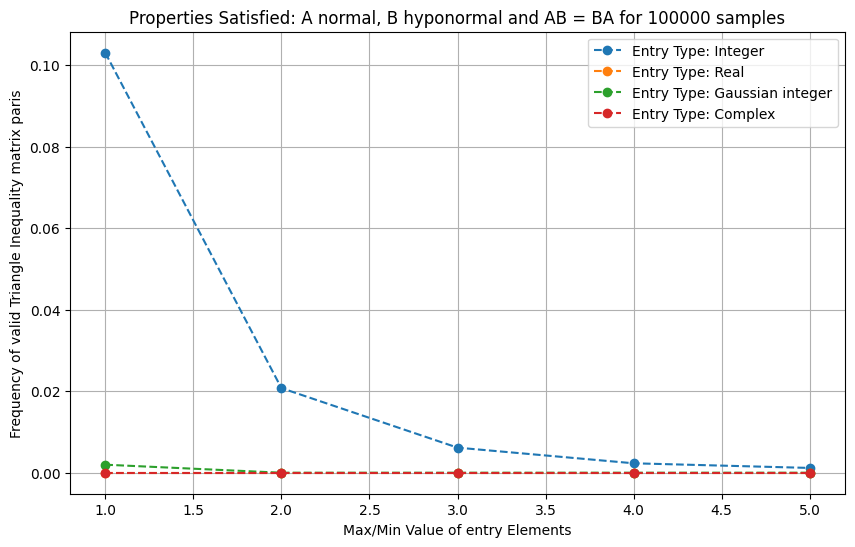
\includegraphics[scale = 0.6]{assets/theorem1plot.png}
    \caption{Random search method for matrix pairs that satisfy Theorem \ref{theorem2} for $A, B \in \mathbb{M}_2.$}
\end{figure}


\par Another case where the triangle inequality will always pass is when:
\begin{theorem}[Mortad \cite{Mortad}] %Theorem 3.15 in Mortads paper
    \label{theorem3} 
    Let $A, B \in \mathbb{M}_n(\mathbb{F})$ such that:
    \begin{enumerate}
        \item $AA^* = A^*A$ (Normal)
        \item $AB = BA$ \text{(Commutative)}
        \item $A^*B + B^*A \leq 0$,
    \end{enumerate}
     \text{ then:} $|A+B| \leq |A|+|B|$
\end{theorem}


\begin{example}[Using Theorem \ref{theorem3}]
    Consider: 
    $$
    A = \begin{bmatrix}
        -1 & 0 \\ 0 & -1
    \end{bmatrix} \quad
    \text{and} \quad
    B = \begin{bmatrix}
        0 & -1 \\ 1 & 1
    \end{bmatrix}
    $$
    Clearly $A$ and $B$ commute, and checking the inequality results in:
    \begin{align*}
        A^*B + B^*A &=
        \begin{bmatrix}
            -1 & 0 \\ 0 & -1
        \end{bmatrix}
        \begin{bmatrix}
            0 & -1 \\ 1 & 1
        \end{bmatrix} + 
        \begin{bmatrix}
            0 & 1 \\ -1 & 1
        \end{bmatrix}
        \begin{bmatrix}
            -1 & 0 \\ 0 & -1
        \end{bmatrix}\\
        &= 
        \begin{bmatrix}
            0 & 1 \\ -1 & -1
        \end{bmatrix} + 
        \begin{bmatrix}
            0 & -1 \\ 1 & -1
        \end{bmatrix}\\
        & = 
        \begin{bmatrix}
            0 & 0 \\ 0 & -2
        \end{bmatrix}\\
        &\leq
        \begin{bmatrix}
            0 & 0 \\ 0 & 0
        \end{bmatrix}
    \end{align*}
    Then the triangle inequality is guaranteed to succeed. We verify with the results with the following:
        $
        |B| = 
        \begin{bmatrix}
            \frac{2\sqrt{5}}{5} & \frac{\sqrt{5}}{5} \\
            \frac{\sqrt{5}}{5} & \frac{3\sqrt{5}}{5}
               \end{bmatrix}
        $
    and $ |A+B| = \begin{bmatrix}
        \frac{3\sqrt{5}}{5} & \frac{\sqrt{5}}{5} \\
            \frac{\sqrt{5}}{5} & \frac{2\sqrt{5}}{5}
    \end{bmatrix}$
    and with
    \begin{align*}
        |A|+|B|-|A+B| &= \begin{bmatrix} 
            1-\frac{\sqrt{5}}{5}& 0 \\ 0 & 1 + \frac{\sqrt{5}}{5}
        \end{bmatrix}\\
        &\approx
        \begin{bmatrix}
            0.553 & 0 \\ 0 & 1.447
        \end{bmatrix}\\
        &\geq
        \begin{bmatrix}
            0 & 0 \\ 0 & 0
        \end{bmatrix}.
    \end{align*}
    This shows that it passes.
\end{example}


The exhaustive search method for integer entries between $-1$ and $1$ found $377$ pairs which satisfies this new theorem resulting \(11.5\%\) of these pairs
making up the population of total successes.
When increasing the integer entry range to $-2$ and $2$ there are $4145$ matrix pairs which satisfy Theorem \ref{theorem3} resulting these pairs making up approximately $2.5\%$ of total successes.
As this entry range increases further the frequency of these matrix pairs falls below $1\%$.
Once again the random search method for integers mirrors the results of the exhaustive with a sample size of $100,000$ is used.
When the matrix is populated with complex integers there is approximately $3.3\%$ of these matrix pairs with the entry range of $-1$ to $1$.
Increasing the entry range with these matrices resulted with the frequency decreasing to less than $1\%$.
The real field and complex field both result with $0\%$ for all entry ranges tested, however as previously discussed, is likely due to an artifact. 
\begin{figure}[H]
    \centering
    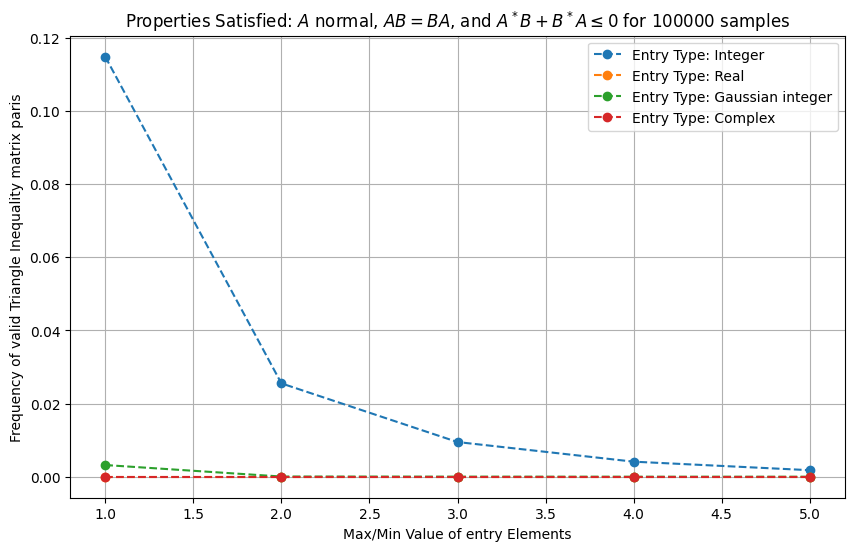
\includegraphics[scale = 0.6]{assets/theorem2plot.png}
    \caption{Random search method for matrix pairs that satisfy Theorem \ref{theorem3} for $A, B \in \mathbb{M}_2.$}
\end{figure}
\par Matrices in higher dimensions for Mortad's theorems were examined using the random search method only due to hardware limitations. The amount of matrix pairs that satisfied
these theorems was found to be negligible when compared with pairs which inherently satisfy the triangle inequality since Mortad's pairs make up less then \(1\%\) of them in \(\mathbb{M}_3\) and \(0\%\)
for \(\mathbb{M}_n\),  \(n \geq 4 \). In \(\mathbb{M}_3(\mathbb{Z} \cap \{ -1, 0, 1\} )\) the frequency for Theorem \ref{theorem2} is approximately \(0.03\%\) and for Theorem \ref{theorem3} it is
\(0.13\%\). Comparing these frequencies shows that there are more than four times the amount of pairs in Theorem \ref{theorem3} than in Theorem \ref{theorem2}. This behavior was present in \(\mathbb{M}_2\)
also and would suggest that there are more matrix pairs for Theorem \ref{theorem3} for which the triangle inequality is valid for \(\mathbb{M}_n\) than pairs found in Theorem \ref{theorem2}.

\par While Mortad's \cite{Mortad} theorems give some reasons for when the triangle inequality is valid, these pairs are very sparse in their contribution to the to set of valid matrix pairs
which satisfies the triangle inequality. 